%=========================================================================
% (c) 2011, 2012 Josef Lusticky

\chapter{Implementation}
This chapter describes an implementation of the designed interface improvements
and an implementation of the designed NTP client application.
How to get a working setup with Contiki on this platform is described in
the document files on the CD enclosed to this thesis.
The CD content hierarchy is listed in appendix~\ref{app:cd-content}.

%Since there is no way of setting, getting and adjusting the time in Contiki OS,
%the interface for setting, getting and adjusting time was developed in this thesis.

\section{Time specification structure}
New structure for expressing time values was implemented.
This structure is similar to POSIX {\it{timespec}} structure,
as described in section~\ref{sec:analysis-interface}.
However, name was chosen {\it{time\_spec}} to avoid collision with
existing POSIX-compliant systems.
\begin{lstlisting}
struct time_spec {
  long sec;
  long nsec;
};
\end{lstlisting}
This structure consists of two signed long values for expressing seconds and nanoseconds.
The value 0 seconds and 0 nanoseconds is equal to Unix prime epoch (1st January 1970).
In case of seconds part, the 32-bit signed long value was chosen because
it can conveniently
represent real-time values as well as local clock adjustment values, which may also be negative.
Such a time representation will wrap around in year 2038 and is facing
what is commonly known as the year 2038 problem~\cite{posix}.

In case of nanoseconds part, the 32-bit signed long value was chosen because
one second has $10^9$ nanoseconds and it is
desirable to be able to express positive as well as negative values for local clock adjustments.
As 32-bit signed long type shall be able to express values from -$2^{31}$-1 (-2~147~483~647)
to $2^{31}$-1 (2~147~483~647)~\cite{c99},
such representation will therefore never wrap around.

It should be noted that signed long data type does not have to always result in a 32-bit variable -
it is up to compiler what data width it chooses for each data type.
But as ISO C99 standard states, the maximum value for an object of type signed long
shall be greater or equal $2^{31}$-1 (2~147~483~647)~\cite{c99}.
This in fact results in at least 32-bit variable unless the compilation setting is changed.
Next to this, the already presented variable {\it{seconds}} is of unsigned long type,
the value {\it{sec}} in the {\it{time\_spec}} structure %and {\it{boottime}}
shall be therefore of the same data width.

Usage of unsigned data type delays the wrap around problem to year 2106,
but will disable use of negative values needed for adjusting local clock.
Since the current NTP Era ends in 2036,
the NTP client application code has to be changed in the future~\cite{ntp-y2k}.

\section{Setting the time}
Setting the current time is only possible within one second precision -
finer time setting must be made using the time adjustments.
Implemented {\it{clock\_set\_time}} function computes when the system started
in seconds since the Epoch and saves the result in the newly implemented {\it{boottime}} variable.

Not only no variables incremented every interrupt nor any internal clock registers
are affected, but also already presented variable {\it{seconds}} is not modified.
Modifying this variable would lead to misbehaviour of stimer library
described in section~\ref{sec:contiki-timers}.

Thanks to this newly implemented {\it{clock\_set\_time}} function and {\it{boottime}} variable,
running Contiki system is able to tell uptime, current time and time when was the system booted.
\begin{lstlisting}
volatile unsigned long boottime;

void
clock_set_time(unsigned long sec)
{
  boottime = sec - seconds;
}
\end{lstlisting}

%%%
\section{Getting the time}
Getting the correct current time is only possible if it was set using
the {\it{clock\_set\_time}} function before.
Newly implemented function {\it{clock\_get\_time}} is then able to tell the
current time in seconds since the Epoch by simply adding {\it{boottime}},
and {\it{seconds}}.

Nanoseconds part is filled in by reading the {\it{scount}} variable and the counter register {\it{OCR2A}}.
Since the counter register can be of a different name on another AVR CPU
and the clock interface is common for all AVR CPUs,
a new general name {\it{CLOCK\_COMPARE\_REGISTER}} was defined in the {\it{clock\_init}} setup code
for the compare register {\it{OCR2A}}.
Similarly, the {\it{CLOCK\_COMPARE\_REGISTER}} was defined for the counter register {\it{TCNT2}},
the default value of the clock compare register was defined as {\it{CLOCK\_COMPARE\_DEFAULT\_VALUE}}
and the {\it{CLOCK\_CTC\_MODE}} was defined as 1, since the hardware clock is used in CTC mode,
which adds one counter register increment as described in section~\ref{sec:analysis-interface}.

The comparison avoids the need to disable clock interrupts for an atomic
read of the multi-byte variable and it is a common solution of the race conditions
on AVR platfroms in Contiki described in~\ref{sec:design-clock}.
\begin{lstlisting}
void
clock_get_time(struct time_spec *ts)
{
  uint8_t counter, tmp_scount;
  do {
    ts->sec = boottime + seconds;
    do {
      counter = CLOCK_COUNTER_REGISTER;
      tmp_scount = scount;
    } while (counter != CLOCK_COUNTER_REGISTER);

    ts->nsec = tmp_scount * (1000000000 / CLOCK_SECOND) +
               counter * (1000000000 / (CLOCK_SECOND * (CLOCK_COMPARE_DEFAULT_VALUE + CLOCK_CTC_MODE)));
  } while(ts->sec != (boottime + seconds));
}
\end{lstlisting}
Because {\it{1000000000}} and {\it{CLOCK\_SECOND}} are both constants, the compiler is able to
calculate the result of division during compile time.
Furthermore as both numbers are integers, the result is integer as well~\cite{c99}.
The most of the CPU time is therefore spent on multiplication where the variables
{\it{counter}} and {\it{tmp\_scount}} are involved.
E.g. if the code is compiled using GCC version 4.3.5,
multiplication of two 32-bit variables takes 33 instructions including {\it{call}} and {\it{ret}}
instructions for entering and returning from the {\it{\_\_mulsi3}} routine, which computes
the result of a multiplication.
According to AVR Instruction Set manual~\cite{avr-instruction-set},
such a multiplication results in 48 clock cycles overhead,
which takes 6~000 nanoseconds assuming 8~MHz CPU clock.
The timestamp provided is therefore not exact.
However, since the consumed time strongly depends on architecture and compiler specifications,
no correction was implemented to remove this inaccuracy.
The application must be instead aware that the timestamp is not exactly accurate.

\section{Adjusting the time}
A new call computing the amount of needed adjustments was implemented.
The {\it{clock\_adjust\_time}}
%Adjusting time
%1/128/32 = 0.000244141
%0.000244141x32x127+0.000244141x31 == smallest possible adjustment == 244us

Time values that are between two consecutive non-negative integer multiples
of the resolution of the specified clock are truncated down to the smaller multiple of the resolution.

%=========================================================================
% (c) 2011, 2012 Josef Lusticky

\section{NTP client code}
The client itself is implemented as a Contiki process.
Parameters such as remote port, local port or poll interval
can be configured using standard C define macro.
The client can communicate using both,
the NTP broadcast mode and the NTP unicast mode.
The unicast mode can be turned off by specifying no remote host.

Structure representing NTP message was borrowed from OpenNTPD daemon
and Dragonfly NTP daemon.
This structure is not using the GCC extension for representing a bit field,
instead uses a single 8-bit integer called {\it{status}}
for Leap Indicator, Version Number and Mode fields of NTP packet
described in section~\ref{sec:ntp-network}.
Accessing each field of the {\it{status}} byte is done using bitmasks.
Unlike using the bit field extension,
such a design is compliant with the standard C language.


%Even if {\it{tmpts.sec}} value is greater than {\it{ts.sec}} value,
%subtracting and casting to signed type gives correct (negative) result~\cite{c99}.
%Assuming 32-bit data types this will work until 2038 when wrap around can occur due to difference
%between {\it{ts.sec}} and {\it{tmpts.sec}} greater than $2^{31}$-1 (2~147~483~647).
%But as NTP Era 0 ends 2036 the NTP client code must be changed in the future anyway~\cite{ntp-y2k}.

%! TODO

%Adjusting time
%1/128/32 = 0.000244141
%0.000244141x32x127+0.000244141x31 == smallest possible adjustment == 244us

%% SENDING NTP TIMESTAMP
The transmit timestamp sent by the client can be set to any arbitrary value.
This is in compliance with the NTPv4 specification~\cite{rfc5905}.
It is however important for the client to store the sent timestamp,
since it is later used by the client to check the server's response.
Contiki NTP Client fills and checks only the seconds part of NTP timestamp,
because the timestamp should be as accurate as possible and the
conversion from nanoseconds to NTP fraction part would increase the interval
between determination of the timestamp and dispatch of the packet.

After the filled NTP packet is sent, the client schedules
sending of a next NTP packet in $2^{\tau}$ seconds
using the event timer library.
In NTPv4, $\tau$ ranges from 4, resulting in poll interval 16 seconds,
to 17, resulting in poll interval 36 hours.
However, the event timer library imposes a limit to scheduled time.
This limit is platform specific and depends on {\it{CLOCK\_SECOND}} value.
The $\tau$ value can not be greater than 8 on AVR Raven assuming 128 interrupts per second.
Upon scheduling the event timer, the client process yields
and another process can be run.
The client process is later invoked either by the uIP stack event
announcing the server response
or by the event timer in case no server response arrived.
Event timer is therefore effectively
dealing with possible packet loss described in section~\ref{sec:design-network}.

When the server response arrives,
determinating the destination timestamp is one of the first thing the client does.
After that, the client makes packet sanity tests including
checking whether the response is from synchronised server.

A determination of the NTP communication mode follows.
In unicast mode, the seconds field of Originate timestamp
is compared with the stored sent timestamp.
The received packet is considered bogus in case of mismatch and further processing is stopped.
Otherwise are the NTP timestamps converted to local timestamp format and
the local clock offset computed as described in section~\ref{sec:ntp-algorithms}.
After the local clock offset is computed,
the stored transmitted timestamp is immediately set to zero
to protect against replay of the last transmitted packet.

In broadcast mode, the received packet is always considered correct
and the local clock offset is computed as the difference between the local stored timestamp
and the transmit timestamp received.
As one could expect, the local clock offset determined from the broadcast mode
is less accurate then from the unicast mode.

Due to a different origin of the Unix and NTP epoch,
number of seconds between NTP and Unix epoch,
is subtracted from seconds part of NTP timestamp.
But the conversion from fraction part of long 64-bit NTP timestamp to nanoseconds,
used in the local timestamp structure,
is one of the most problematic tasks for memory constrained systems.
An accurate conversion requires either floating point operations or operations with 64 bit numbers.
The conversion is given by
$nsec = fractionl \times 10^9 \div 2^{32}$, where $nsec$ is the nanoseconds part of the local timestamp
and $fractionl$ is the fraction part of long 64-bit NTP timestamp.
Since there is no native hardware support for floating point nor for 64-bit arithmetic,
GCC would supply these operations in form of library called {\it{libgcc}},
which causes significantly bigger resulted binary file.
The greatest common divisor of $10^9$ and $2^{32}$ is $2^9$,
so in fact, a relatively simple multiplication of $fractionl$ by $\frac{5^9}{2^{23}}$ must be computed.
This can be computed using sequential divisions and multiplications,
which in turn can be done on 32 bits using shifts and additions~\cite{c99}.
\begin{lstlisting}[caption=Conversion from NTP fraction part to nanoseconds]
unsigned long
fractionl_to_nsec(uint32_t fractionl)
{
  unsigned long nsec;
  nsec = fractionl;
  nsec = (nsec >> 1) + (nsec >> 3); // nsec = nsec/2 + nsec/8 = (5*nsec)/8
  nsec = (nsec >> 1) + (nsec >> 3); // nsec = (5*nsec) / 8 = (25*fractionl)/64
  nsec = (nsec >> 1) + (nsec >> 3); // nsec = fractionl * 5^3/2^9
  /* Now we can multiply by 5^2 because then the total
   * multiplication coefficient for the original number fractionl
   * will be: fractionl * (5^5)/((2^3)^4) = fractionl * 0.762939453,
   * which is less then 1, so it can not overflow.
   */
  nsec = (nsec << 1) + nsec + (nsec >> 3); // nsec*3 + nsec/8 = (25*nsec) / 8

  nsec = (nsec >> 1) + (nsec >> 3);
  nsec = (nsec >> 1) + (nsec >> 3);

  /* Again we can multiply by 5^2.
   * Total coefficient will be fractionl * (5^9)/((2^3)^7) = fractionl * 0.931322575
   */
  nsec = (nsec << 1) + nsec + (nsec >> 3); // nsec*3 + nsec/8 = (25*nsec) / 8

  /* Last shift to agree with division by 2^23 can not be
   * done earlier since the coefficient would always be greater than 1.
   */
  nsec = nsec >> 2;
  return nsec;
}
\end{lstlisting}
As the code comments say, an extra attention must be taken of the overall
multiplication coefficient,
that can not be greater than 1 in any step.
Because $fractionl$ can be of any value between $0$ and $2^{32}-1$,
the overall coefficient greater than 1 could cause overflow and an unexpected result.

According to output from the {\it{avr-size}} tool,
when compiled with GCC 4.3.5,
using the 64-bit arithmetic for conversion
takes 656 bytes more in %program section of
resulted binary file (GCC supplies routine for multiplication and shifting 64-bit integers)
and floating point operation takes 3~358 bytes more
than the developed algorithm.

It must be noted, that the above presented conversion is not exactly accurate, particularly
because of loosing the least significant bits by the first shifts.
However, this conversion gives maximum error of 5 nanoseconds for all possible values of $fractionl$,
which is totally adequate for most platforms without floating point unit or
for platforms where usage of 64-bit arithmetic is expansive.
Beside significantly smaller memory requirements,
this algorithm gives on AVR Raven even more accurate results than the libgcc
floating point library supplied by GCC.


In the next step after conversions, the local clock offset is computed
as given in section~\ref{sec:ntp-algorithms}.
Depending on the absolute value of the local clock offset,
the system time is either set or adjusted using the {\it{clock\_set\_time}}
and {\it{clock\_adjust\_time}} call respectively.
The clock is set if the time difference is equal or greater than
treshold value, which 3 seconds by default. %!TODO
The reference NTP implementation uses 125 ms~\cite{rfc5905}
It has been the Internet
experience that the need to change the system time in increments
greater than +-128 ms is extremely rare and is usually associated
with a hardware or software malfunction or system reboot~\cite{rfc1589}.


%
% NEGATIVE result for the first time
%In some scenarios where the initial frequency offset of the client is
  %relatively large and the actual propagation time small, it is
   %possible for the delay computation to become negative.  For instance,
   %if the frequency difference is 100 ppm and the interval T4-T1 is 64
   %s, the apparent delay is -6.4 ms.  Since negative values are
   %misleading in subsequent computations, the value of delta should be
   %clamped not less than s.rho, where s.rho is the system precision
   %described in Section 11.1, expressed in seconds~\cite{rfc5905}.
%


%=========================================================================
% (c) 2011, 2012 Josef Lusticky

\section{Network communication}
% 1 - see design/network.tex
Communication over IEEE~802.15.4 link layer uses a 6LoWPAN adaptation layer.
Thanks to this layer, AVR Raven running Contiki OS is connected to the IPv6 Internet.
The client and the developed interface uses no IP version specific code,
therefore a communication over IPv4 should be also possible, though not tested.

The packet loss problem was described in section~\ref{sec:design-network}.
However, packet loss is not a matter for NTP if using either broadcast or unicast mode.
In broadcast mode, lost server packet causes no setting or adjusting time of client's
local clock.
The client simply waits without disruption for next NTP broadcast message.
If client needs to figure out it's local clock offset at the moment,
it can simply query a server using NTP unicast mode.
% 2
Upon sending the packet, the NTP client process yields
using the {\it{PROCESS\_YIELD}} statement, so no active waiting
causes blocking the whole system.

The remote NTP server can be specified in Makefile or
using the {\it{REMOTE\_HOST}} define macro.
If no remote host is specified,
NTP client assumes only NTP broadcast communication mode will be used.
The broadcast mode is intended particularly for energy or memory constrained clients
or for a huge number of NTP clients and a single NTP server
in a network with small propagation delay.
Should there be more devices running Contiki present in one network,
each of them needs a different link layer address.
This address can be configured in Makefile as well.
Beware that the firmware for RZ~USB Stick automatically translates % sice
between Ethernet link layer addresses (MAC addresses) and IEEE~802.15.4 link layer
addresses, but both are are still different links and can not be used in one
%physical
network topology.

Dynamic increasing or decreasing the client's poll interval in response to
Kiss-o'-Death packets, described in section~\ref{sec:ntp-network}, is not implemented.
The configuration instead assumes, that an exhausted NTP server rather drops the incoming
client's packet than sending the response with KoD code.

Contiki NTP Client is primarily intended for use in local networks with a single master NTP server,
although using any NTP server found in the Internet would work.
Figure~\ref{fig:implementation-routing} shows the network topology used
for tests and measurements of Contiki NTP Client.
% How to set up the illustrated network is described in tutorial on CD.
The Meinberg primary NTP server was synchronised with PPS %todo.
Measurements made using this setup are discussed in chapter~\ref{chap:measurements}.

\begin{figure}
	\centering
	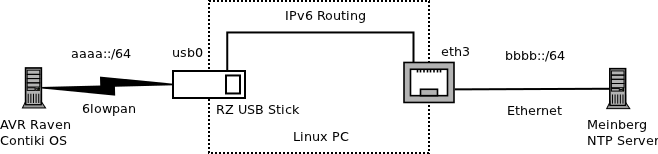
\includegraphics[width=10cm,keepaspectratio]{fig/radvd-routing.png}
	\caption{Contiki NTP Client communicating with remote NTP server}
	\label{fig:implementation-routing}
	%\bigskip
\end{figure}


%=========================================================================
% (c) 2011, 2012 Josef Lusticky

\section{Code metrics}
The patch improving the Contiki operating system version 2.5
inserts 175 new lines of code and modifies 1 line of code.
The modified line is a backport from the actual Contiki Git version to prevent
missing the compare match between the {\it{scount}} variable and {\it{CLOCK\_SECOND}} value.

The patch improving the actual Contiki operating system Git version at the time of writing,
inserts 78 lines of code and modifies 1 line of code.
The modified line fixes a reported bug, which has not been fixed at the time of writing.
This bug causes a bad decision of the C preprocessor whether the {\it{CLOCK\_SECOND}}
value is a power of two, which in turn may cause a division operation in
the clock interrupt service routine.

The NTP client application has 2 code files and 1 header file.
The code file containing the definition of the NTP process
has 198 lines of code.
The second code file contains only various conversions from NTP fraction part
to nanoseconds.
The user may choose using the C define macro which conversion will be used
by the NTP client application.
This file has 52 lines of code.

Various code metrics of the NTP client application code
shows listing~\ref{lst:implementation-metrics}.
These metrics were acquired using the {\it{cloc}} program.
\begin{lstlisting}[caption={NTP client application code metrics},label={lst:implementation-metrics}]
-----------------------------------------------------------------------------
Language                   files          blank        comment           code
-----------------------------------------------------------------------------
C                              2             52            122            198
C/C++ Header                   1             19             54             52
-----------------------------------------------------------------------------
SUM:                           3             71            176            250
-----------------------------------------------------------------------------
\end{lstlisting}

